\chapter{Database Design}
\label{ch:database-design}

\section{Overview}

\noindent PostgreSQL~17 is the single primary database, accessed exclusively
through the Drizzle ORM. The schema is defined in TypeScript in
\texttt{packages/database/src/schema} and deployed as 48 generated SQL
migration files. The current schema contains 47 relations, grouped into the
four families rendered below: (1) identity, tenancy, authentication, and
authorization; (2) academic structure, materials, content, and material
intelligence; and (3) questions, examination, practice, and operational
sub-systems (jobs, OCR registry).

\section{Family 1: Identity, Tenancy, Authentication, and Authorization}

\noindent Figure~\ref{fig:erd-identity} shows the tenancy and authorization
core. Key design properties:

\begin{itemize}
  \item \textbf{Tenant anchor.} \texttt{users} join \texttt{institutes}
  through \texttt{memberships}; a membership is unique per
  (user, institute) and carries an active/deactivated status. All feature
  tables reference \texttt{institute\_id}.
  \item \textbf{Session-bound authentication.} \texttt{auth\_sessions} store a
  SHA-256 hash of the refresh token, an expiry, a revocation timestamp, and a
  \texttt{rotated\_from\_sid} self-link that records rotation lineage.
  \texttt{password\_resets} stores only the bcrypt hash of the one-time secret,
  with a single-use guarantee.
  \item \textbf{Permission catalogue enforced by the schema.}
  \texttt{permissions} rows mirror the typed catalogue in code; \texttt{roles}
  are distinguished as system/institute and institute/platform through CHECK
  constraints and partial unique indexes; \texttt{role\_permissions} and the
  junction \texttt{membership\_roles} implement role-to-permission binding.
  \texttt{\seqsplit{platform\_user\_roles}} binds a user to platform-domain roles,
  fully disjoint from institute membership.
  \item \textbf{Plans.} \texttt{plans} and \texttt{institute\_subscriptions}
  form a minimal lifecycle foundation (starter/growth/institute tiers) without
  billing or feature columns.
\end{itemize}

\begin{figure}[h]
\centering
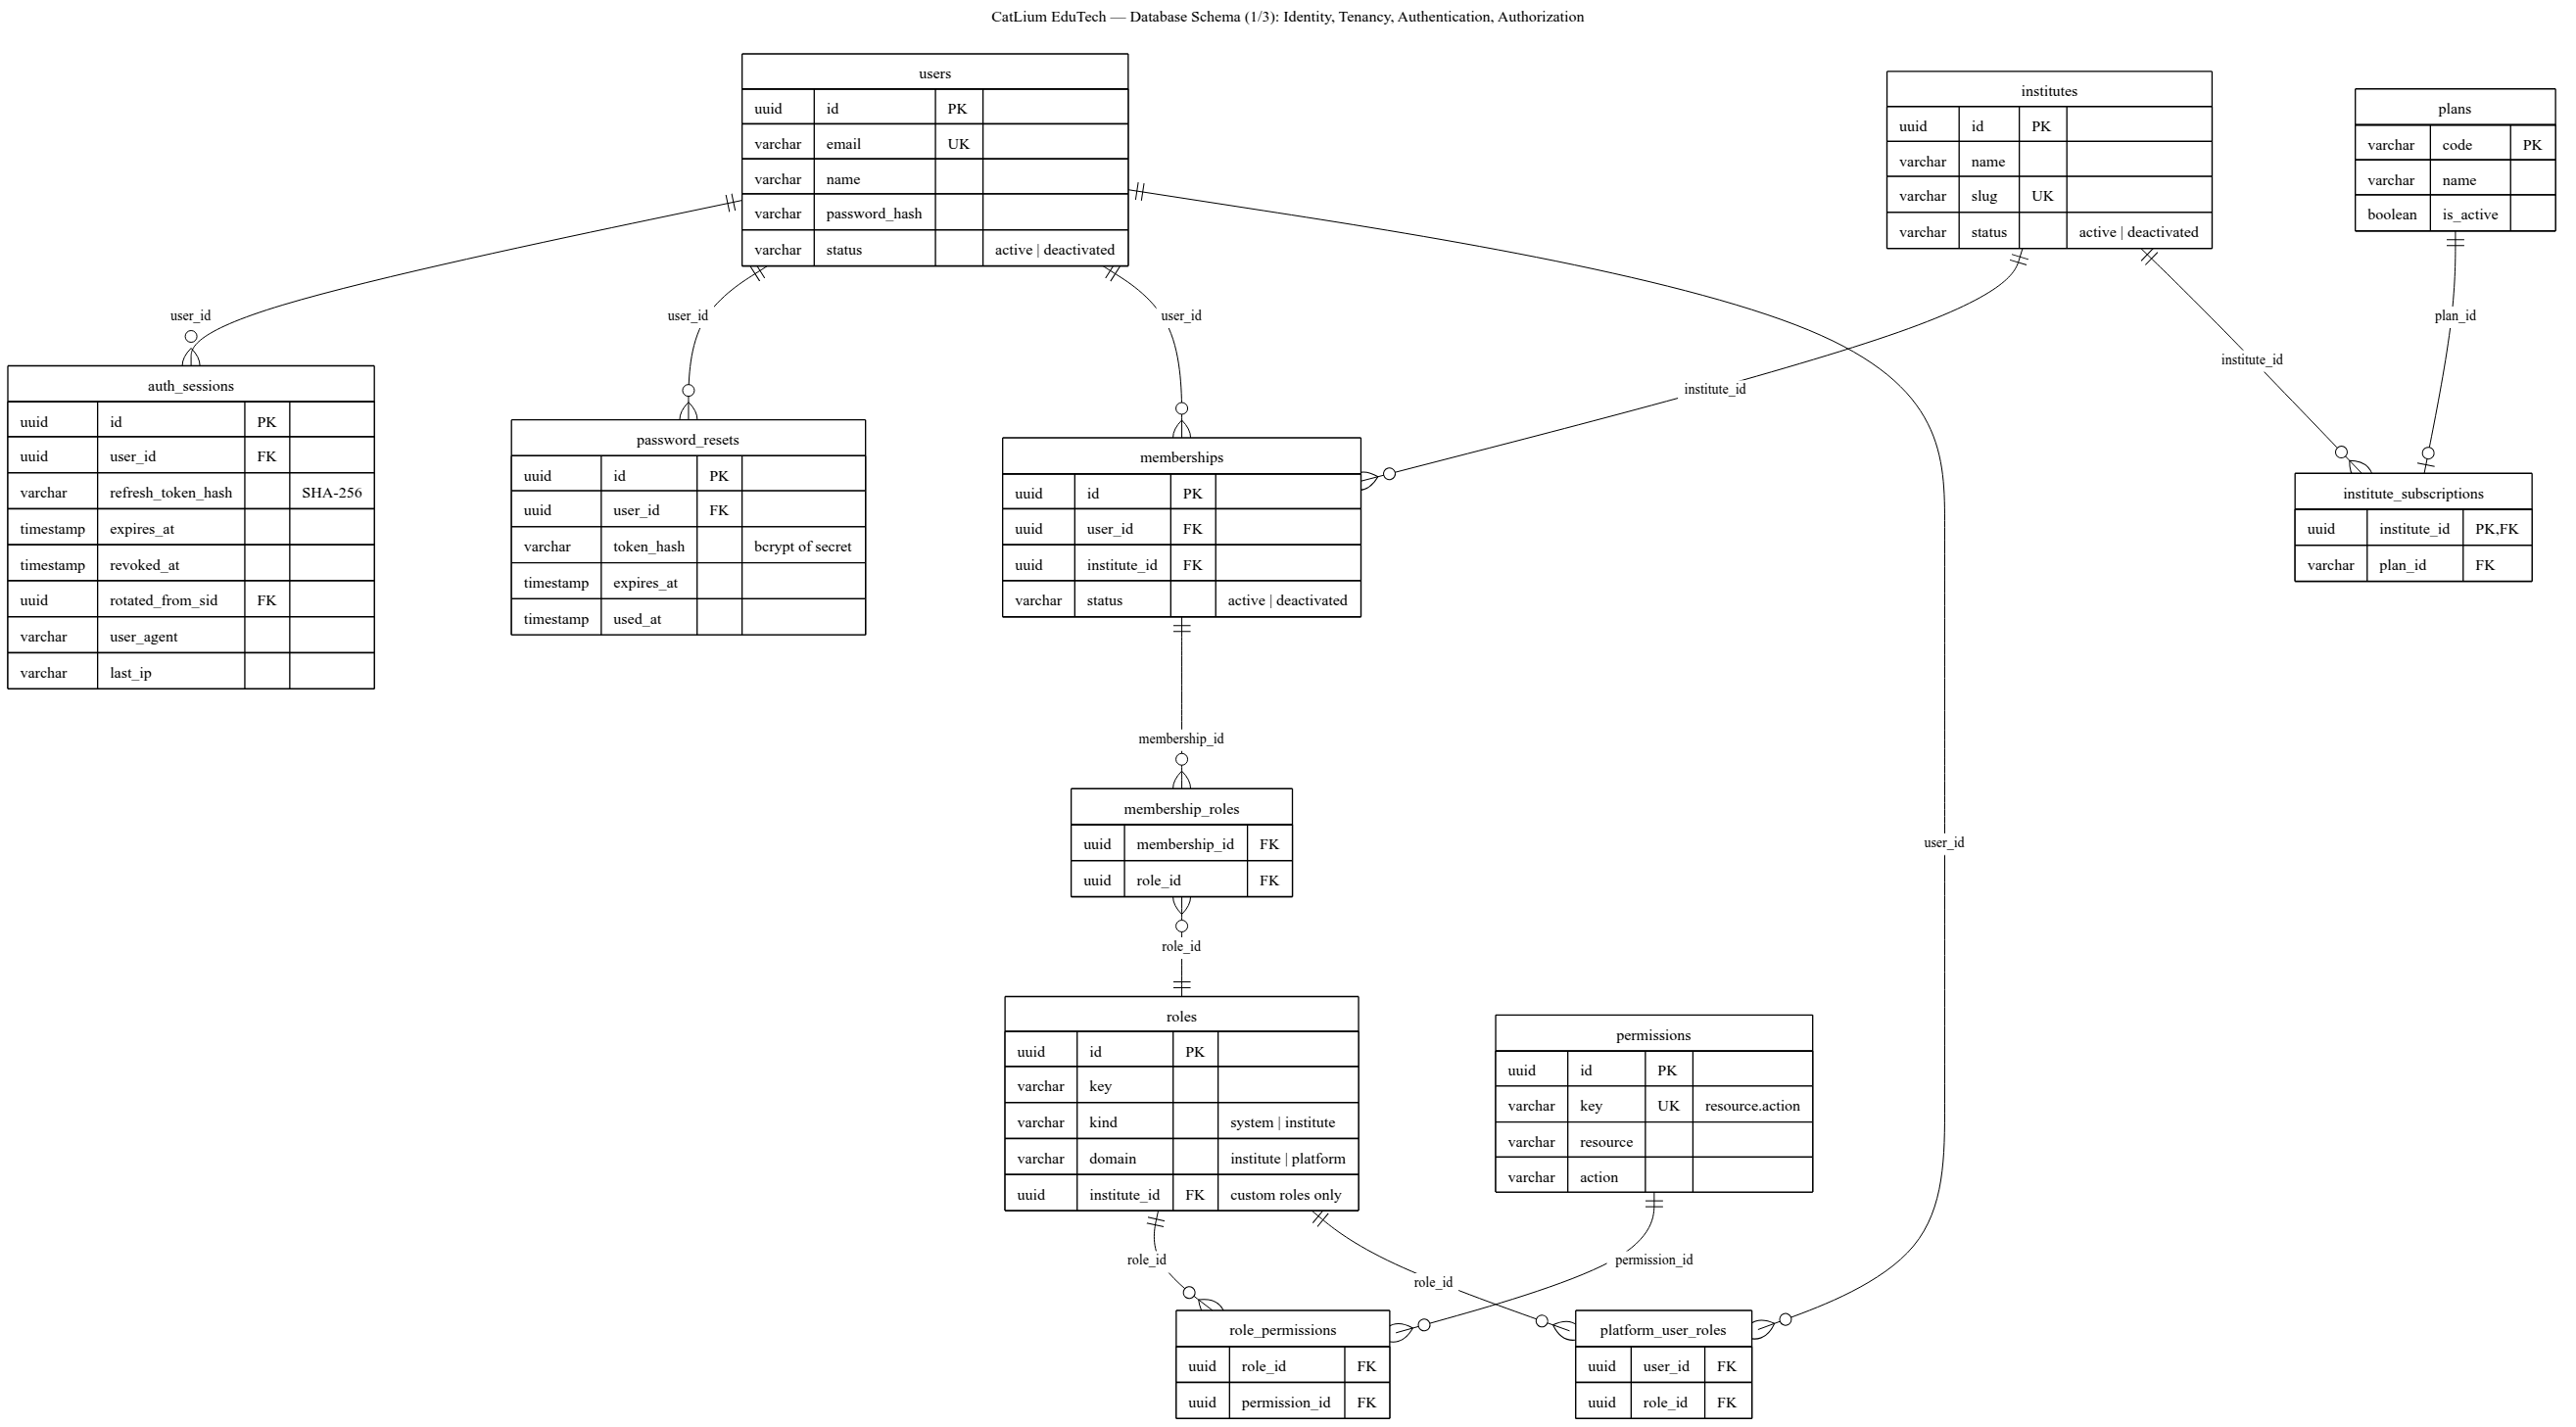
\includegraphics[width=\textwidth]{figures/database-erd-identity-bw.png}
\caption{Database schema --- identity, tenancy, authentication, authorization.}
\label{fig:erd-identity}
\end{figure}

\section{Family 2: Academic Structure, Materials, Content, and Intelligence}

\noindent Figure~\ref{fig:erd-academic-content} shows the academic and
content families. Properties:

\begin{itemize}
  \item \textbf{Scope chain.} \texttt{subjects $\rightarrow$ chapters
  $\rightarrow$ topics} is the single authority for academic scoping; the
  schema enforces consistency with a CHECK on the subject id across the chain.
  \item \textbf{Offerings and assignments.} \texttt{classes} pair with
  \texttt{subjects} in \texttt{class\_subjects} (the offering). Teachers are
  bound to offerings through \texttt{teacher\_assignments}; students are
  placed into a year--class--division through \texttt{student\_placements} and
  may override the inherited subject set with
  \texttt{\seqsplit{student\_subject\_enrollments}} (\texttt{ENROLLED} /
  \texttt{EXCLUDED}).
  \item \textbf{Material vs content.} \texttt{materials} are uploaded
  artifacts with a processing lifecycle and a storage key;
  \texttt{content\_items}/\texttt{content\_versions} are derived, versioned
  study resources whose payload is stored as JSONB with rendered HTML and AI
  context. \texttt{material\_enhancements} (with segment and segment-mapping
  children) store the deterministic structural enrichment of a material.
  \item \textbf{Soft delete.} \texttt{subjects} keeps a nullable
  \texttt{deleted\_at} so academic structure can be archived without
  destroying references.
\end{itemize}

\begin{figure}[h]
\centering
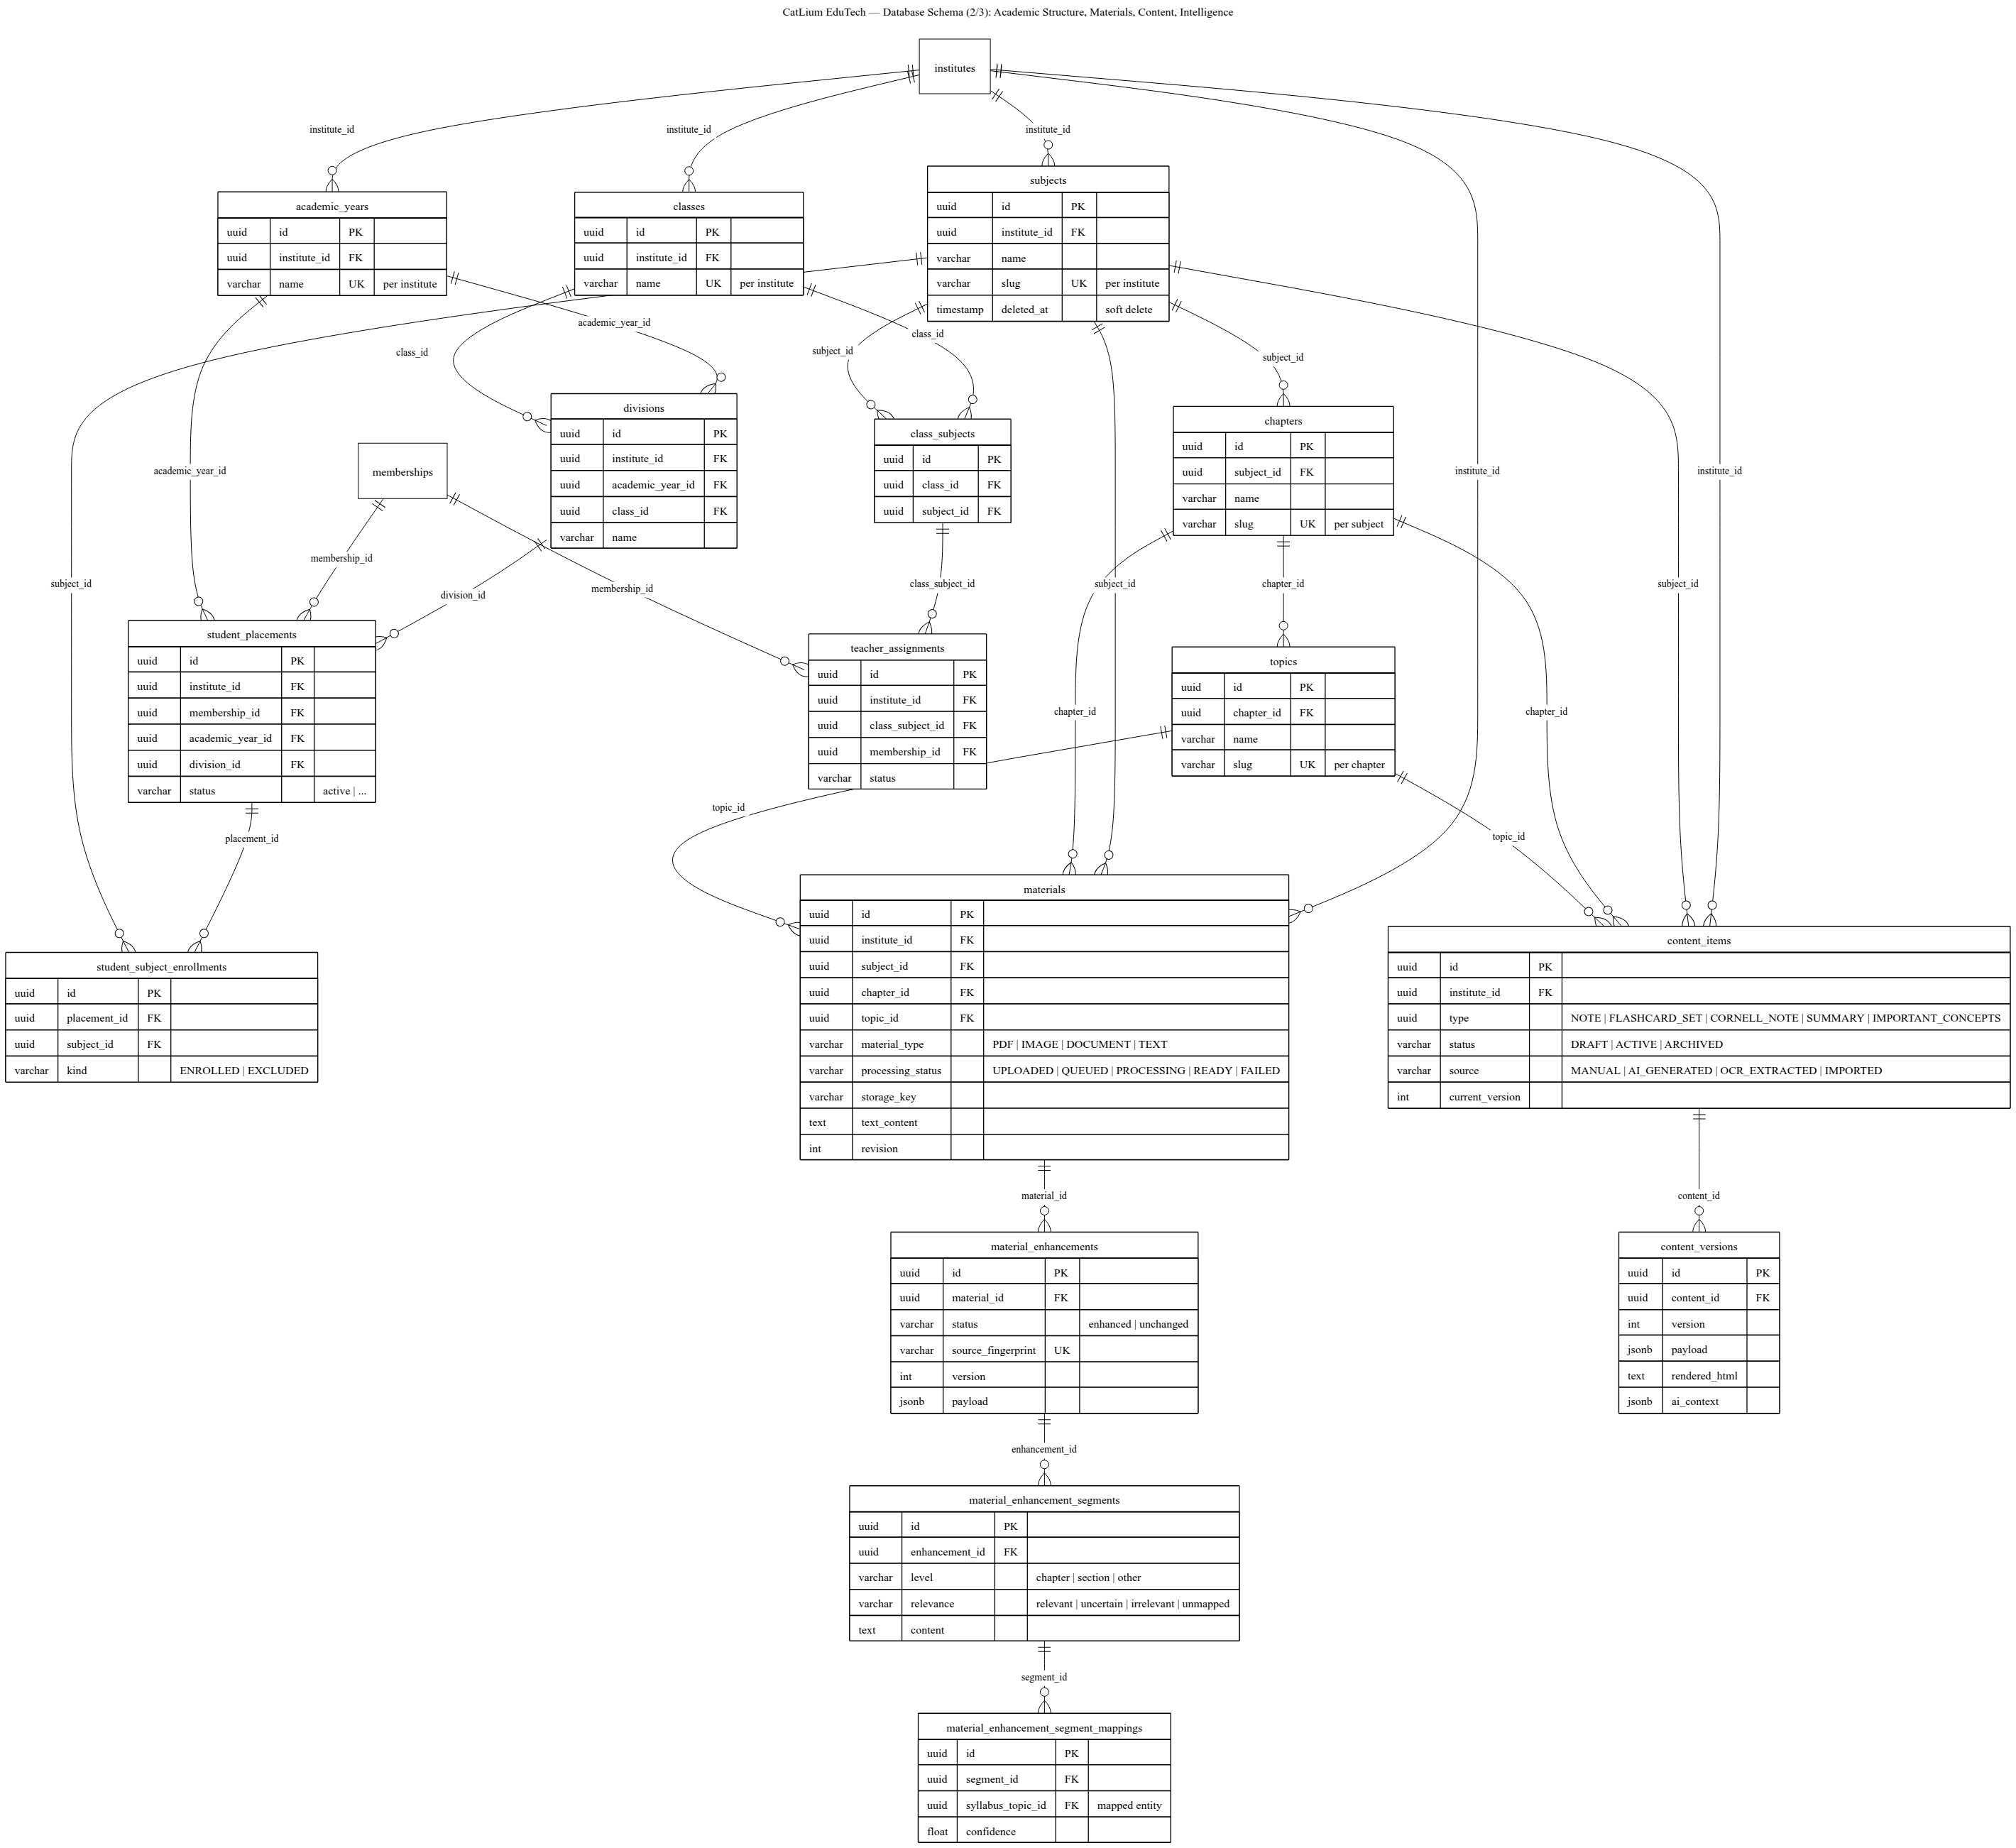
\includegraphics[width=\textwidth]{figures/database-erd-academic-content-bw.png}
\caption{Database schema --- academic structure, materials, content, and
material intelligence.}
\label{fig:erd-academic-content}
\end{figure}

\section{Family 3: Questions, Examination, Practice, and Operations}

\noindent Figure~\ref{fig:erd-operations} shows the question, examination,
practice, and operational families. Properties:

\begin{itemize}
  \item \textbf{Question types as data.} \texttt{question\_types} holds 11
  seeded global starter types plus institute-custom types; \texttt{code} is
  the stable key and \texttt{answer\_format} is copied onto every
  \texttt{questions} row at write time.
  \item \textbf{Immutable attempt snapshot.} \texttt{attempts} records a
  terminal-with-evaluation invariant; \texttt{attempt\_questions} snapshots
  the question stem, type, format, marks, and full server-side payload at
  attempt start; \texttt{attempt\_responses} is the upsertable answer with
  \texttt{is\_correct} and \texttt{marks\_awarded}.
  \item \textbf{Paper artifacts.} \texttt{paper\_patterns} (with
  \texttt{paper\_pattern\_subjects}) drive selection into
  \texttt{question\_papers} and \texttt{assessments} through dedicated
  junction tables that freeze marks, sections, and sort order.
  \item \textbf{Practice.} \texttt{practice\_sessions} support two modes via
  a mode column, and their items/responses are snapshot-like; answers are
  stored with a rating or a correctness flag, never a score.
  \item \textbf{Operational registry.} \texttt{jobs} carries status,
  payload, requester, and completion time with a partial unique index that
  prevents duplicate active AI-generation jobs per source.
  \texttt{workers}/\texttt{ocr\_chunks} implement the distributed OCR
  coordination, with chunk status, \texttt{claimed\_by}, lease expiry, and an
  attempt counter.
\end{itemize}

\begin{figure}[h]
\centering
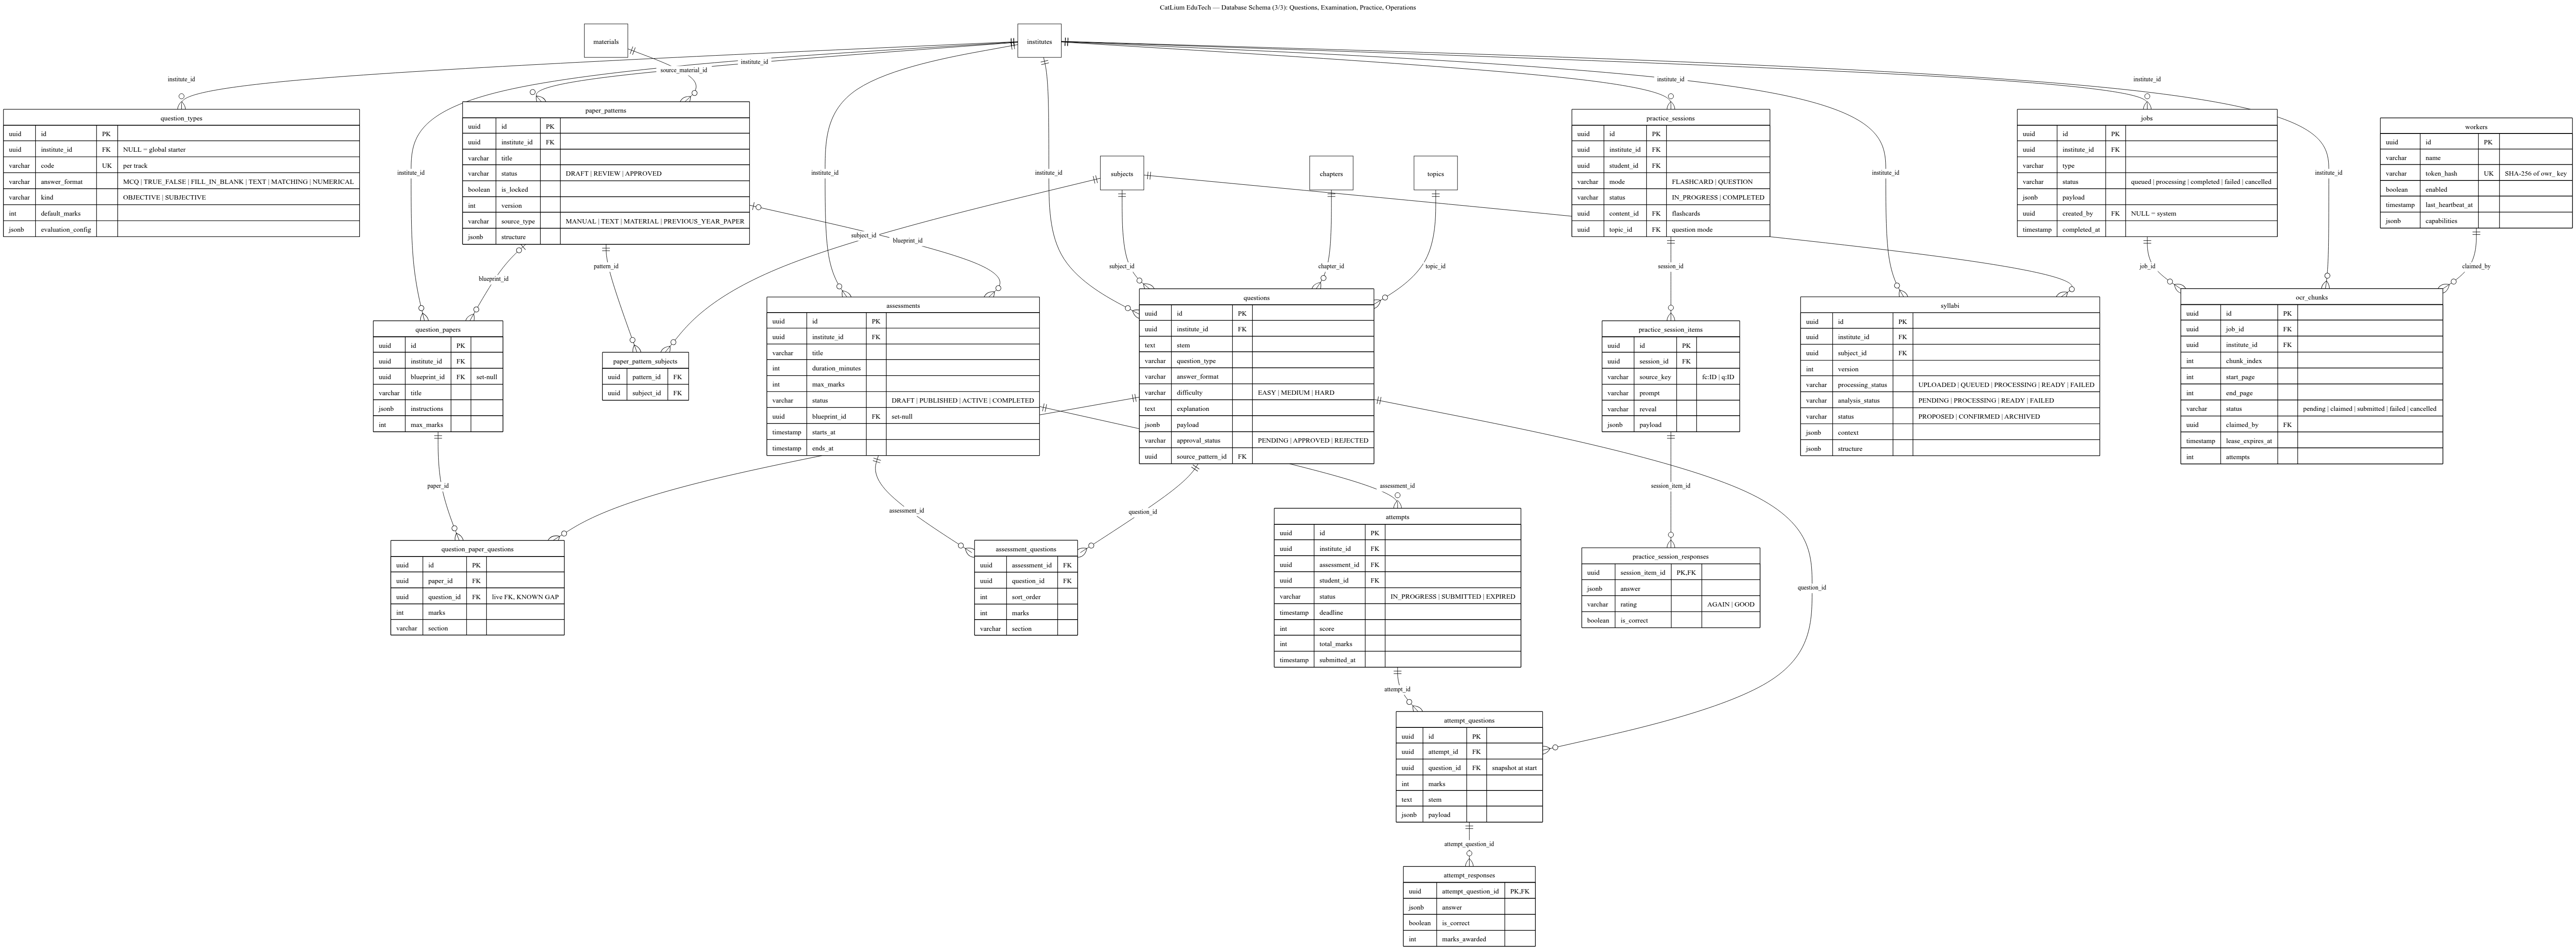
\includegraphics[width=\textwidth]{figures/database-erd-operations-bw.png}
\caption{Database schema --- questions, examination, practice, and operations.}
\label{fig:erd-operations}
\end{figure}

\section{Design Principles Applied}

\noindent Four principles recur across all 47 relations:

\begin{enumerate}
  \item \textbf{Tenant scoping at the row.} Every table that can hold user or
  institute data carries \texttt{institute\_id} so that a forced WHERE clause
  is always available.
  \item \textbf{JSONB for flexible payloads.} Structured-but-variable content
  (question payloads, paper structures, syllabus structures, AI context,
  job payloads) is stored as JSONB and validated at the boundary by Zod
  (TypeScript) or Pydantic (Python), keeping the relational core stable.
  \item \textbf{Snapshot over reference where evaluation depends on it.}
  Attempt question items, practice items, and question-paper junctions copy
  the fields they depend on, so later edits to a source question cannot
  silently change an in-flight or historical artifact.
  \item \textbf{Database-enforced invariants.} Partial unique indexes (one
  in-progress attempt per assessment+student, one open practice session per
  source, no duplicate active generation per source) turn races into
  deterministic \texttt{409} conflicts; \texttt{FOR UPDATE SKIP LOCKED} makes
  the OCR chunk claim safe under concurrency.
\end{enumerate}